\documentclass[9pt,twocolumn,twoside]{gsajnl}
% Use the documentclass option 'lineno' to view line numbers
\usepackage{booktabs}
\usepackage{siunitx}
\usepackage{adjustbox}
\usepackage{geometry}
\articletype{gos} % article type

\title{Nucleotide Diversity Loss on a Plant Y Chromosome Following Recent Recombination Suppression}

\author[$\ast$,$\dagger$,1]{Josh Hough}
\author[$\dagger$]{Wei Wang}
\author[$\dagger$]{Spencer C.H. Barrett}
\author[$\dagger$]{Stephen I. Wright}

\affil[$\ast$]{Department of Plant Sciences, University of California, Davis}
\affil[$\dagger$]{Department of Ecology and Evolutionary Biology, University of Toronto}

%\affil[$\dagger$]{Author two affiliation}
%\affil[$\ddagger$]{Author three affiliation}
%\affil[$\S$]{Author four affiliation}
%\affil[$\ast\ast$]{Author five affiliation}

\keywords{Sex Chromosome Evolution; Nucleotide Diversity; Recombination; Deleterious Mutations}

\runningtitle{Plant sex chromosome evolution} % For use in the footer

\correspondingauthor{Josh Hough}

\begin{abstract}
X and Y chromosomes differ in effective population size ($N_{e}$), rates of recombination, and exposure to natural selection, all of which can affect levels of genetic diversity. On Y chromosomes with suppressed recombination, selection is expected to eliminate neutral variation and reduce the $N_{e}$ of Y compared to X chromosomes or autosomes. However, non-selective factors including female biased sex ratios and high variance in male reproductive success can also reduce Y-linked $N_{e}$, making it difficult to infer the causes of low Y-diversity. Here, we investigate the factors affecting levels of polymorphism within the genome during sex chromosome evolution in \textit{Rumex hastatulus} (Polygonaceae), a dioecious plant with young sex chromosomes. Strikingly, we find that neutral diversity for genes on the Y is on average \textasciitilde 2.1\% of the value for their homologues on the X, corresponding to a chromosome-wide reduction of \textasciitilde 93\% compared to the neutral expectation. We demonstrate that the magnitude of this diversity loss is inconsistent with a reduced male $N_{e}$ caused by neutral processes including female-biased sex ratios and high variance in male reproductive success. Instead, using forward simulations, we show that the loss of diversity on the Y can be explained by interference among a large number ($\geq$ 800 Kb) of weakly selected mutations. Our results are in agreement with theory on "interference selection", and provide evidence that the effects of purifying selection over a large number of genetically-linked sites can substantially reduce neutral diversity. Given the recent origin of \textit{R. hastatulus} sex chromosomes (\textasciitilde 15MYA), our results imply that Y chromosome degeneration in the early stages may be largely driven by interference rather than positive selection for gene silencing followed by neutral genetic drift.
\end{abstract}


\setboolean{displaycopyright}{true}

\begin{document}

\maketitle
\thispagestyle{firststyle}
\marginmark
\firstpagefootnote
\correspondingauthoraffiliation{jhough@ucdavis.edu}
\vspace{-11pt}

\section*{Introduction}

\lettrine[lines=2]{\color{color2}M}{}orphologically distinct sex chromosomes have evolved multiple times independently in both plants and animals \citep{westergaard1958,ohno1967,bull1983,charlesworth1991,charlesworth2015plant}. Despite clear biological differences between these kingdoms, X and Y chromosomes in both lineages have undergone similar genetic changes. For example, in both groups the loss of recombination between X and Y chromosomes has been associated with an accumulation of deleterious mutations and a gradual loss of genes from the Y chromosome \citep{hough2014,bergero2015,bachtrog2013NRG}, and in some species, the degeneration of the Y has led to the evolution dosage compensation of the X chromosome \citep{charlesworth1996CB,muyle2012,mank2013sex,papadopulos2015}. The independent evolution of these phenomena in such taxonomically distant species suggest that general evolutionary mechanisms may be involved, but inferring the causes of molecular evolution and patterns of polymorphism in genomic regions that lack recombination is a longstanding challenge for both theoreticians and experimentalists \citep{charlesworth1978,feldman1980evolution,barton1995general,charlesworth1996CB,otto1997deleterious,charlesworth2000degeneration,mcvean2000effects}.

One fundamental difference between the X and Y chromosomes is that there are 1/3 as many Y-linked gene copies as X-linked ones in a diploid population. Thus, genes on the Y chromosome are expected to experience an effective population size ($N_{e}$) that is 1/4 that of autosomal genes, whereas the  $N_{e}$ for genes on the X chromosome should be 3/4 that of autosomal genes (assuming an equal number of reproducing females and males). The lowered $N_{e}$ of the Y chromosome implies that that the equilibrium level of neutral polymorphism - proportional to the product of $N_{e}$ and the neutral mutation rate, $\mu$ - should be lower for Y-linked genes than for their X-linked counterparts. In the absence of recombination, genes on the Y chromosome are also expected to be in strong linkage disequilibrium, making them vulnerable to diversity loss due to selection against strongly deleterious mutations (background selection) and selective sweeps of strongly beneficial mutations (genetic hitchhiking). Furthermore, the build-up of linkage disequilibrium between selected mutations on the Y means that selection will act non-independently across the chromosome such that selection at a focal site may "interfere" with selection at sites with which it is linked. Originally developed by Hill & Robertson (1966), a large body of work has now shown that such "selective interference" can substantially reduce both the efficacy of selection and the level of neutral variability \citep{fisher1930genetical, muller1964relation, hill1966HReffect, mcvean2000}. These arguments all suggest that non-recombining Y chromosomes should harbor a lower amount of neutral genetic variability than predicted based on the number of Y chromosomes in a population, but the extent to which background selection, genetic hitchhiking, or selective interference have affected chromosome-wide levels of diversity in natural populations, and the relative importance of these processes, is not well-understood.

In addition to reduced diversity arising from selection, in species with female-biased sex ratios or extensive male-male competition, high variance in male reproductive success is also expected reduce the $N_{e}$ experience by genes on the Y chromosome \citep{caballero1995,charlesworth2001,laporte2002,pool2007,ellegren2009}, suggesting that inferences about the effects positive of purifying selection need to be distinguished from these neutral processes. Because variance in male reproductive success reduces both Y-linked $N_{e}$ and autosomal $N_{e}$ \citep{kimura1964number,nomura2002effective}, evidence for this can therefore be obtained by comparing levels of neutral diversity on X and Y chromosomes relative to values on autosomes. For example, high variance in male reproductive success causes a reduction in the Y/A diversity ratio, but an increase in the X/A ratio. Based on such comparisons, studies in humans, for example, have suggested that the inflated X/A ratio is attributable to a historical excess of breeding females over males \citep{hammer2008sex} (and see \citep{bustamante2009,hammer2010,cotter2016genetic}).

Despite widespread interest in determining the evolutionary factors affecting neutral diversity on sex chromosomes \citep{ellegren2011,bachtrog2013NRG}, we know very little about the influence of either sex ratio variation or linked selection in determining levels of diversity on more recently evolved sex chromosomes. The time scales over which these different effects are likely to be important is therefore not well understood. In humans, estimates of Y-linked diversity are considerably lower than predicted under neutral models, and simulations suggest that levels of diversity are consistent with strong purifying selection \citep{Wilsonsayres2014}. However, given that human sex chromosomes evolved from autosomes \textasciitilde 200 million years ago (MYA), is not immediately obvious whether purifying selection might have such strong effects on Y chromosomes that evolved \textit{do novo} from autosomes over much more recent evolutionary time (e.g., within the last 20 MYA in the case of plants \citep{charlesworth2015plant}). Y-linked diversity loss might on the one hand be expected to be lower in younger systems due to a shorter history of recombination suppression. On the other hand, simulations of strong selection models (background selection and genetic hitchhiking) suggest that these processes may have the greatest effects during the earliest stages of sex chromosome evolution, before the Y has lost many of its genes \citep{bachtrog2008temporal}. Moreover, work by \citep{KaiserCharlesworth} and \citep{good2014genetic} have provided evidence that even weak purifying selection, if acting non-independently across large number of sites, can generate substantial deviations from neutrality, whereas classic background selection theory breaks down in such cases. Given that a large number of sites are likely to be in linkage disequilibrium on a recently evolved Y chromosome, such "interference selection" \textit{sensu} \citep{good2014genetic} is a good candidate model for exploring the evolutionary dynamics of young plant sex chromosomes.

To investigate the factors affecting nucleotide diversity in the early stages of sex chromosome evolution, we analyzed neutral polymorphism levels on X, Y, and autosomal chromosomes in the plant \textit{R. hastatulus }(Polygonaceae). This species is a dioecious annual with heteromorphic X and Y chromosomes that evolved approximately 15 MYA \citep{quesada2011,grabowska2015,navajas2005}, making Y chromosomes in this species over 100 million years younger than the highly degenerated Y chromosomes in mammals \citep{lahn1999,ross2005dna}. \textit{Rumex hastatulus} has also received particular attention because of the occurrence of an intraspecific polymorphism in sex chromosome system, in which both XY and $XY_{1}XY_{2}$ males occur in geographically distinct populations ("chromosomal races") \citep{smith1963mechanism}. The $XY_{1}XY_{2}$ sex chromosome system in this species is thought to have originated through an X-autosome fusion, with the XY system maintaining the ancestral chromosome complement \citep{smith1964evolving}. Despite the recent origin of sex chromosomes in both races, there is evidence that both Y's have undergone significant gene loss and functional deterioration \citep{hough2014}. Here, to simplify our comparison of polymorphism levels on X, Y, and autosomes, we focus only on the ancestral Y chromosome, which occurs in both sex chromosome races.

Of particular importance for our study, \textit{R. hastatulus} populations have been found to consistently exhibit female-biased reproductive sex ratios, with a mean sex ratio of $N_{f}/(N_{m}+N_{f})=0.6$ \citep{pickup2013influence}. Female-biased sex ratios are not uncommon in dioecious plants with heteromorphic X and Y chromosomes \citep{field2013comparative,hough2013evolutionarily}, and their occurrence in \textit{R. hastatulus} provides an excellent opportunity to study both the demographic and selective factors contributing to sex-linked variability.

\section*{Materials and Methods}
\subsection*{Population Samples and Sex-Linked Genes}
We analyzed sex-linked and autosomal genes identified from Illumina RNA sequence data from 12 males and 12 females (1 male and 1 female from each of 6 populations). Samples were collected in 2010 from throughout the native range of \textit{R. hastatulus} (locations in Table S1), and plants were grown in the glasshouse at the University of Toronto from seeds collected from open-pollinated females. We extracted RNA from leaf tissue using Spectrum Plant Total RNA kits (Sigma-Aldrich). Isolation of mRNA and cDNA synthesis was conducted according to standard Illumina RNAseq procedures, and sequencing was conducted on two Illumina HiSeq lanes with 150-bp end reads at the Genome Quebec Innovation Center. Reads from these samples were mapped to the \textit{R. hastatulus} reference transcriptome \citep{hough2014} using the Burrows–Wheeler Aligner \citep{li2010fast}, followed by Stampy \citep{lunter2011stampy}. We used Picard tools (http://picard.sourceforge.net) to process mapping alignments for the Genome Analysis Toolkit \citep{mckenna2010genome} variant calling software, and subsequently removed genes with low coverage (<10x) and low Phred Quality Scores <20. The population samples analyzed here were previously reported in Hough et al. (2014), where they were used to validate the ascertainment of sex-linked genes identified through segregation analysis, and raw sequences are available from the GenBank Short Read Archive under accession no. SRP041588. Here, to consider sex linked genes that were identified in all of our sequenced population samples, we focused on the previously described set of 460 X/Y genes for which a Y homolog was found in both the Texas and North Carolina races (i.e., X/Y genes where the Y copy was inferred to be on the $Y_{1}$ chromosome).

\subsection*{Autosomal Genes}
In evaluating evidence for nucleotide diversity differences between X and Y chromosomes, it is important to distinguish between reduced Y-linked diversity, and the possibility that X-linked diversity is elevated above the level predicted from a neutral model. To do this, we normalized our sex-linked diversity estimates by autosomal diversity, and compared empirical X/A and Y/A nucleotide diversity ratios to those predicted from neutral models and from simulations (described below). Because the criteria for ascertaining autosomal loci in Hough et al. (2014) were based on identifying four segregating SNPs per locus, and since this set of genes is likely to be higher in diversity than the average autosomal gene, here we instead used the larger set of all non-sex linked (putatively autosomal) genes as our autosomal reference. We filtered genes in this set to remove any genes that may have been sex-linked but were not identified as such by Hough et al.'s conservative ascertainment criteria. In particular, we removed: (i) any genes in which there was evidence for at least one SNP with a sex-linked segregation pattern, (ii) any genes where SNPs showed fixed heterozygosity in males and fixed homozygosity in females, (iii) genes with less than 10X coverage or greater than 100X coverage from independently obtained genomic coverage data (to filter out duplicates or genes with highly repetitive sequences), and (iv) any genes containing SNPs with large (>0.4) allele frequency differences between males and females. Finally, we removed genes with fewer than 100 synonymous sites to avoid biasing our results toward genes that may have been particularly short due to assembly problems. This filtering resulted in a final set of 12,356 autosomal genes.

\subsection*{Phasing X and Y alleles}
To estimate polymorphism for X and Y sequences separately, it is necessary to infer the phase of SNPs in sex-linked transcripts in males. In previous work, phasing alleles on \textit{R. hastatulus} sex chromosomes was achieved using segregation analysis from a genetic cross. Here, to phase SNPs from population samples where such segregation data was unavailable, we used HAPCUT \citep{bansal2008hapcut}, a maximum-cut based algorithm that reconstructs haplotypes using sequenced fragments (Illumina read data) from the two homologous chromosomes to output a list of phased haplotype blocks containing the SNP variants on each chromosome. Because the resulting haplotype blocks produced by HAPCUT contained SNPs that were phased relative to each other, but not designated to either the X or Y chromosome, we assigned individual variants to X or Y by independently identifying fixed X-Y differences within each haplotype block (i.e., sites where all females were homozygous, and all males were heterozygous). Identifying such fixed differences within phased haplotype blocks enabled us to then infer the correct phase (X or Y) of the polymorphisms from HAPCUT’s output. In particular, this was done by matching the phase of fixed X-Y differences with their neighboring polymorphic sites: when a fixed X-Y difference occurred in the same phased haplotype block as a polymorphic site, then the polymorphic variants in that block were assigned to either X or Y based on the known phase of the fixed difference with which they were matched. SNPs that were identified outside of phased blocks, or in blocks without fixed X-Y differences, were recorded as missing data. Finally, we filtered out SNPs with coverage > 60, QUAL score > 60, and those within a distance of 10bp or less from indels. This filtering procedure resulted in fasta-formatted alignments of X and Y sequences for 372 sex-linked genes.

We further validated the results of HAPCUT’s allele phasing by comparing the accuracy of this method with the phasing-by-segregation method that was conducted in Hough et al. (2014). To do this, we first phased the sequence data from parents and their progeny using HAPCUT’s algorithm (using the same parameters as for the population data), and then identified cases where SNPs were inferred on the Y chromosome by HAPCUT, but where the true level polymorphism, obtained from the genetic cross, was zero. We identified 7 \% of sex-linked genes that either had  phasing errors of this kind genotyping errors. This corresponds to a SNP error rate estimate of 1.7 x 10-4. Note that this rate is very low relative to population-based estimates of polymorphism on the X and autosomes (Table 1), and therefore should have minimal effects on our estimation of the X/A ratio. However, because this rate is high relative to the expected level of polymorphism on the Y chromosome, we further filtered genes in which we found evidence for false-positive SNP calls arising from: (i) phasing errors caused by gene duplicates (more than two haplotypes), (ii) polymorphisms around indels, and (iii) genotyping errors caused by low Y-expression. This final filtering was conducted by manually checking each individual putative polymorphism on the Y chromosome using IGV \citep{robinson2011integrative}.

\subsection*{Estimating nucleotide diversity on sex chromosomes and autosomes}
For each locus in our analysis, we calculated Watterson’s (1975) estimator of the population parameter $\theta=4N_{e}\mu$, where $N_{e}$ is the effective population size, and $\mu$ is the mutation rate \citep{watterson1975}, using a modified version of the Perl program Polymorphurama \citep{bachtrog2006}. To compare sex-linked and autosomal loci, we calculated the average value of $\theta$, weighted by the number of synonymous sites in each gene (\X Figure 2). We obtained 95\% confidence intervals for X/A and Y/A ratios by bootstrapping per gene using the BCa method \citep{efron1994} implemented in the Boot package in R \citep{canty2012boot}, and calculating X/A and Y/A on each iteration for 20000 replicates each. Bootstrapping was conducted on the final filtered set of 173 sex-linked, and 12355 autosomal genes. Note that the lack of recombination on the Y chromosome implies that statistical assumptions about independence across loci are violated, suggesting that the true uncertainty in the estimate Y/A may be wider than implied by bootstrapping results. To address this, we also used a maximum likelihood approach, implemented in a modified version of the MLHKA software \citep{wright2004hka}, to independently estimate a credibility interval for the Y/A ratio (Figure S1). Because of the thousands of genes involved, a likelihood method incorporating divergence to control for heterogeneity in mutation rate was not feasible, as this would require maximizing the likelihood estimate of the mutation rate for each locus independently. Therefore, we assumed no heterogeneity in mutation rate, no recombination between Y-linked genes, and free recombination between autosomal loci. Our model thus had two parameters: $\theta_{autosomal}$ and Y/A. We varied both parameters and evaluated the likelihood for Y/A from 0.001 to 1, and $\theta_{autosomal}$ from 0.001 to 0.01.

\subsection*{Neutral predictions and the effect of sex ratio bias on diversity}
To test whether our estimated levels of diversity on X, Y and autosomal chromosomes could be explained by neutral processes, we compared our estimated levels diversity to predictions from a model of the expected $N_{e}$ of males and females when the variance in offpring number is either smaller or larger than Poisson \citep{kimura1964number, hedrick2011genetics}. As we were primarily interested in the possible influence of variance in male reproductive success on Y-linked $N_{e}$, and the parameter space within which such a model might generate Y/A and X/A ratios consistent with our data, we ignored non-poission variance in female offspring, and calculated the male $N_{e}$ as:

\begin{equation}
N_{e_{m}}=\frac{N_{m}k_{m}-1}{k_{m}-1+\frac{V_{k_{m}}}{\overline{k}}} \label{eq:Vk}
\end{equation}

where $k_{m}$ and $V_{k_{m}}$ are the mean and variance in male offspring number, respectively, in a population of $N_{m}$ reproducing males, and $\overline{k}$ is the total mean number of progeny \citep{kimura1964number}. Given expected values of $N_e_{m}$ for a range of values for $V_{k_{m}}$ and $N_{m}$, the corresponding expectation for the $N_{e}$ of autosomes and sex chromosomes at equilibrium were calculated as:

\begin{equation}
N_{e{A}} = \frac{4N_{m}N_{f}}{N_{m}+N_{f}} \label{eq:Ne}
\end{equation}

\begin{equation}
N_{e{X}} = \frac{9N_{m}N_{f}}{4N_{m}+2N_{f}} \label{eq:NeX}
\end{equation}

\begin{equation}
N_{e{Y}} = \frac{N_{m}}{2} \label{eq:NeY}
\end{equation}

following \citep{wright1931evolution}. Note that with equal sex ratios $N_{f} = N_{m}$, and Poisson-distributed offspring numbers ($V_{k} = \overline{k}$), then $N_{e_{X}}/N_{e_{A}} = 0.75$, and $N_{e_{Y}}/N_{e_{A}} = 0.25$. Figure 1 shows these predictions as a function of the sex ratio for a range values of $V_{k_{m}}$, and we tested the fit of our empirical diversity ratios to these predictions (shown in Figure 2) assuming the estimated \textit{R. hastatulus} sex ratio of 0.6 \citep{pickup2013influence}.

\begin{figure}[htbp]
\centering
\noindent
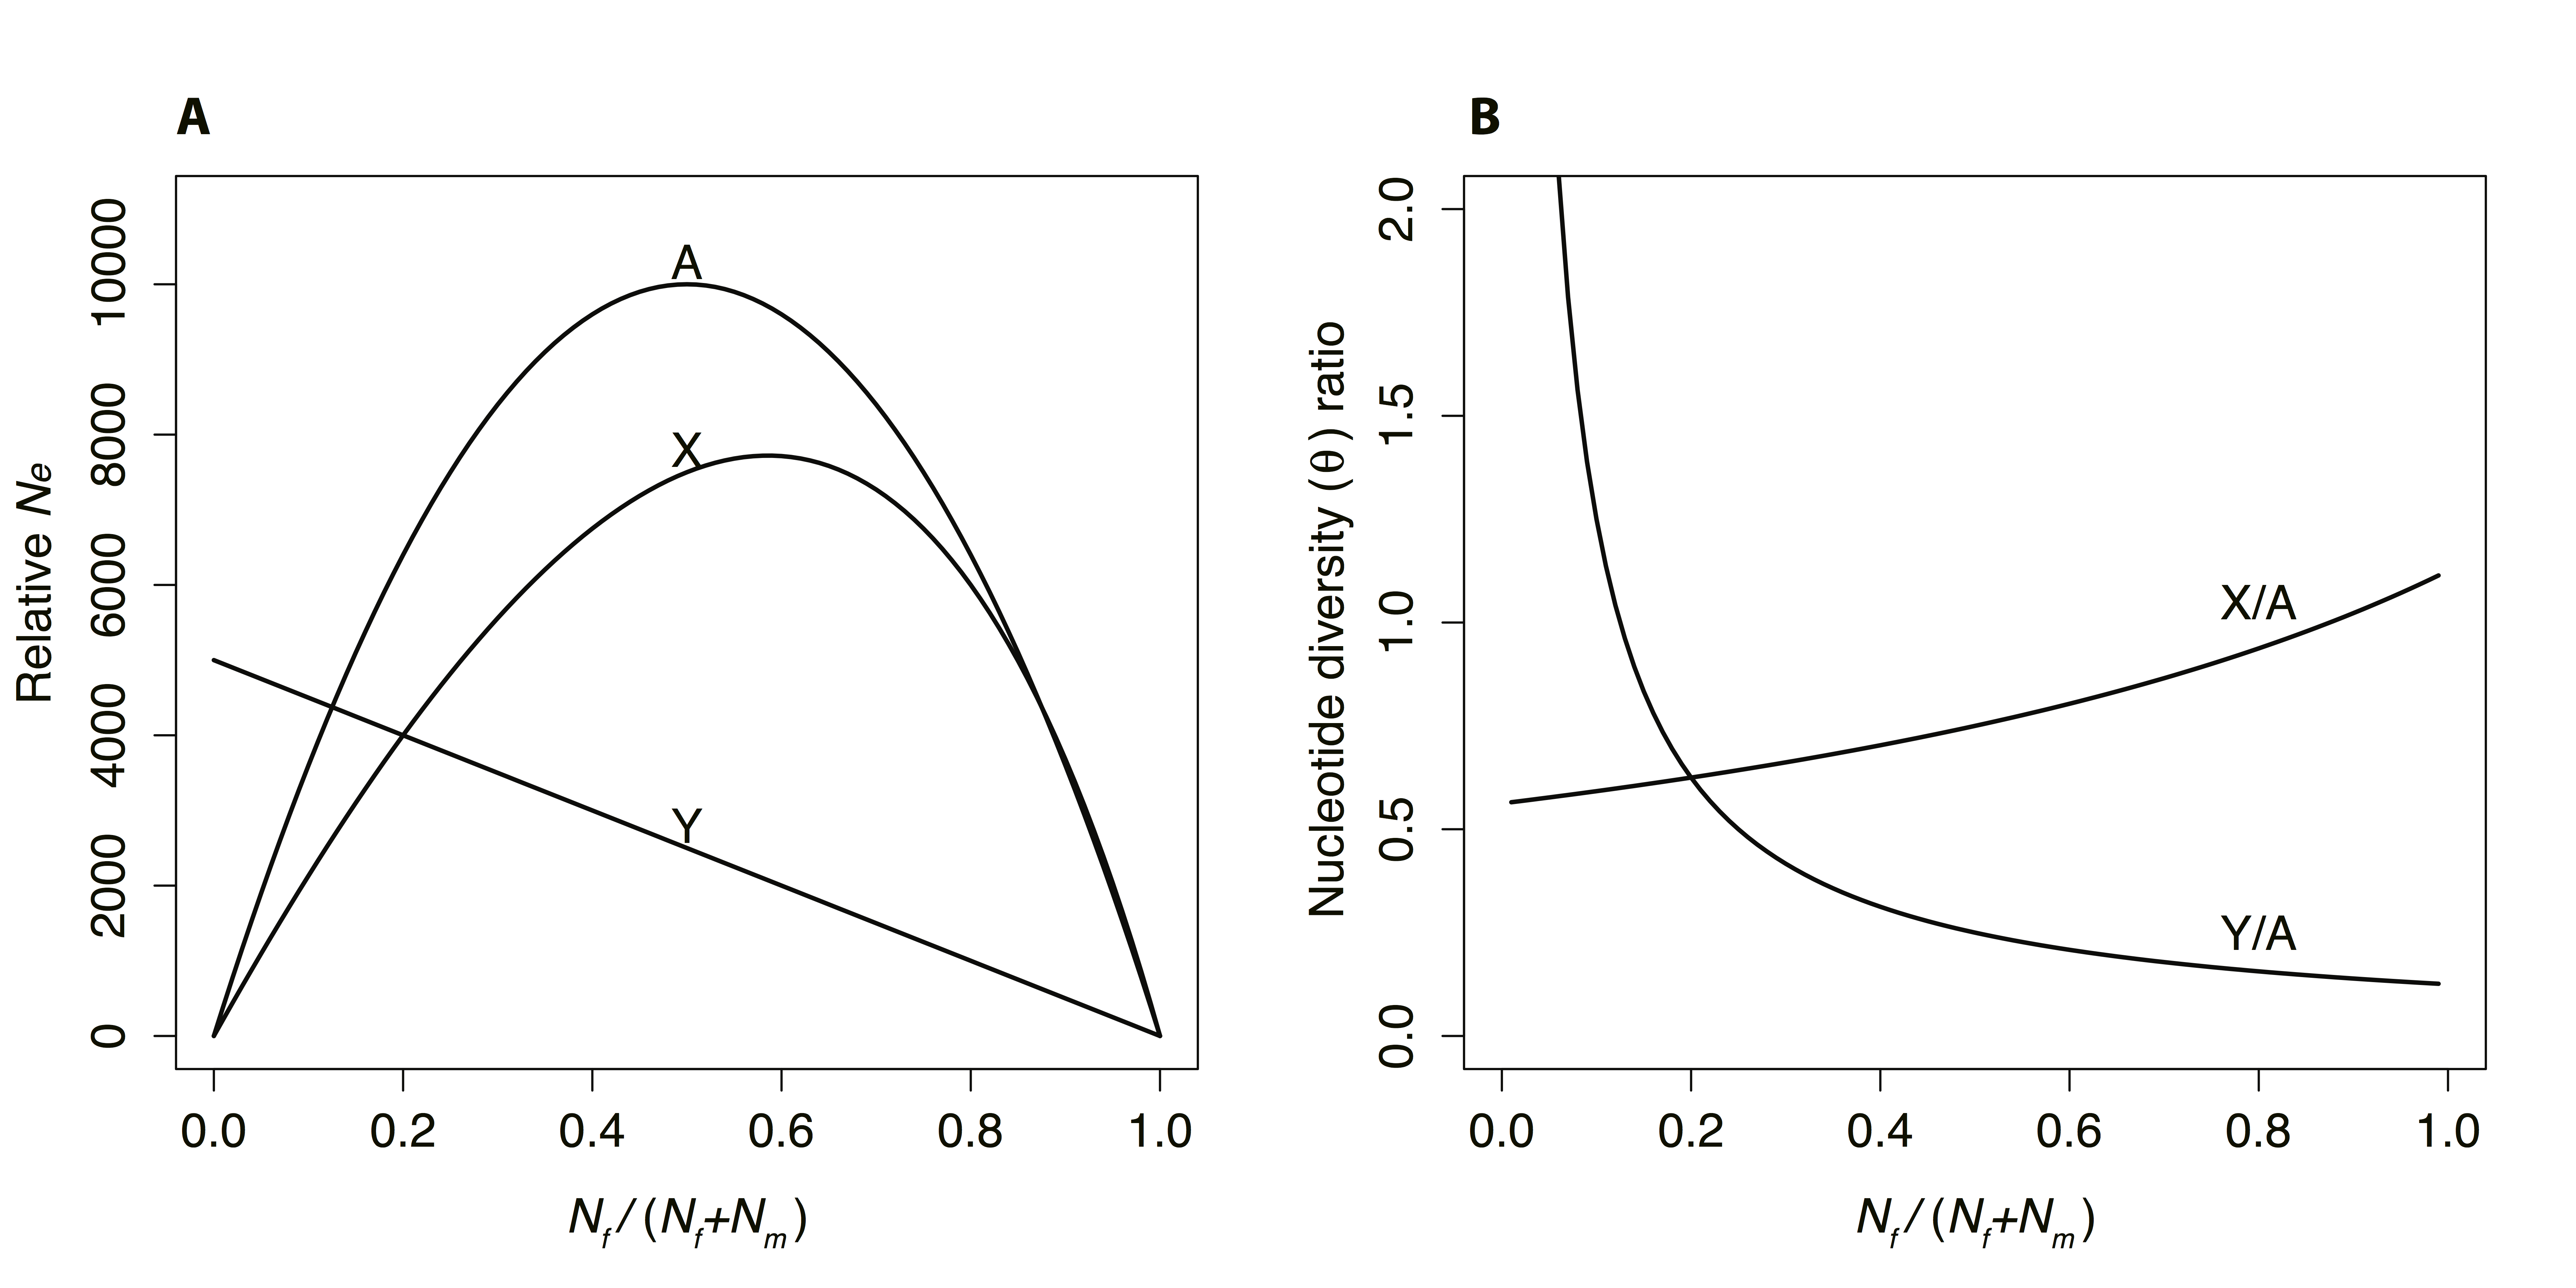
\includegraphics[width=\linewidth]{figure1.jpg}
\caption{The relation between effective population size and sex ratio bias for genes on autosomes (\textbf{A}) and the X chromosome (\textbf{B}), and corresponding normalized X/A and Y/A ratios (\textbf{C}). The sex ratio is shown as the proportion of females, $N_{f}/(N_{f}+N_{m})$, plotted against $N_{e}/N$, where $N=N_{m}+N_{f}$. Dotted curves show equilibrium predictions when both males and females produce Poisson-distributed offspring numbers and ($V_{k}$=$\overline{k}=2$). Solid curves correspond to increasing values for $V_{k_{m}}$, the variance in male offspring number, ranging from Poisson/2 (top solid curve in panels A and B) to 3*Poisson (bottom most curve). For (\textbf{C}) we assumed equal neutral mutation rates among genes and calculated the expected neutral diversity as $\theta=4N_{e}\mu$.
}
\label{fig:spectrum}
\end{figure}

\subsection*{Simulations of purifying selection}
To study the effects of purifying selection on expected levels of Y-chromosome diversity, we used a similar approach to \citep{Wilsonsayres2014} and conducted forward-time simulations of haploid Y chromosomes using the software SFSCODE \citep{hernandez2008flexible}. We first estimated the distribution of fitness effects of deleterious mutations from our polymorphism data for X-linked genes using the method of \citep{keightley2007joint}, which fits a gamma distribution of selection coefficients to the observed frequency distribution of nonsynonymous and synonymous polymorphism. We used this estimated gamma distribution to parameterize the simulations, initializing each with our estimated $\theta$ from autosomal genes, but appropriately adjusted to reflect the expected reduction in Y-linked $N_{e}$ for a sex ratio of $N_{f}/(N_{f}+N_{m})=0.6$. To match our sample size and the number of synonymous sites sample from our data (see Supporting Information), the simulations sampled 6 haploid chromosomes, and simulated sequences contained 45,331bp of linked neutral sequence from which we calculated diversity. To examine the expected reduction in diversity relative to neutrality ($\pi/\pi_{0}$) as a function of the number of selected sites ($L$), and to estimate this parameter from our data, we ran simulations over a range of values of $L$ (up to a maximum of $5x10^{6}$) (Figure 3A). For each simulation, we calculated the approximate likelihood of our observed data based on the proportion of simulations in which synonymous diversity, $\pi_{s}_{simulated}$, matched our empirical estimate, $\pi_{s}_{observed}$ (Figure 3B).

\section*{Results and Discussion}

\subsection*{Extensive loss of Y-chromosome diversity}
Our analysis reveals that diversity on the \textit{R. hastatulus} Y chromosome is significantly lower than expected under neutrality, with estimates indicating Y/A=0.02, ....which is 12.5 fold lower than the standard neutral prediction of Y/A = 0.25 (P<0.0001). We also observe that the Y chromosome shows a 40-fold lower than mean diversity on the X chromosome (Table 1). Note that by normalizing X and Y diversity by autosomal diversity, our results indicate that the X-Y difference we observed was not due to an elevation of X chromosome diversity, but rather a Y-specific reduction. Conceivably, such low diversity on the Y could arise from a low Y-linked mutation rate, or a lower mutation rate in males compared to females. However, these possibilities are unlikely because the number of synonymous mutations in X and Y lineages, estimated by both parsimony and maximum likelihood, are not significantly different \citep{hough2014}. Similarly, our estimates of weighted average synonymous substitution rate between \textit{R. hastatulus} and the outgroup \textit{R. bucephalophorus} reveal similar levels of synonymous divergence at sex-linked (0.2016) and autosomal genes (0.219) \citep{hough2014}.

%After initial analyses revealed a much higher level of diversity on the Y chromosome of the North Carolina race (SUP FIG), we examined evidence for population structure using a Neighbor-joining tree (sup fig). Surprisingly, this analysis revealed that the Y chromosome from this race appears to be paraphyletic, with XYY samples from Florida being more closely related to the TX race than either is to samples from South Carolina (suppfig). Once we examine diversity for these two subclades separately, a strong loss of diversity on the Y chromosome is once again apparent (Table 1).

%Although our sampling of each \textit{R. hastatulus} sub-clade is limited, the discovery of three phylogenetically distinct monophyletic groups is interesting because it suggests the possibility that introgression occurred between the ancestral Texas (XY race) and the derived North Carolina ($XY_{1}Y_{2}$) race, leading to a secondarily-derived $XY_{1}Y_{2}$ sub-clade. As the North Carolina and Texas races are known to be inter-fertile \citep{smith1964evolving}, we suggest that the Florida sub-clade inferred here likely originated through hybridization between a female from the SC clade harboring the X-autosome fusion, and a male from the XY Texas race.


%\begin{table}[htb]
%\centering
%\caption{Estimates of neutral diversity by race on \textit{R. hastatulus} sex chromosomes and autosomes.}
%\begin{tabular}{ccccccccc}
%\textbf{} & \multicolumn{2}{c}{\textbf{Texas}} & \multicolumn{2}{c}{\textbf{South Carolina}} & \multicolumn{2}{c}{\textbf{Florida}} \\
%chromosome & $\theta$ & $\theta/\theta_{A}$ & $\theta$ & $\theta/\theta_{A}$ & $\theta$ & $\theta/\theta_{A}$ \\
%\midrule
%A & 0.006 & 1 & 0.006 & 1 & 0.005 & 1 \\
%X & 0.0047 & 0.85 & 0.0019 & 0.33 & 0.0018 & 0.37 \\
%Y & $\num{e-4}$ & 0.002 & $\num{e-4}$ & 0.002 & $\num{e-4}$ & 0.002 \\
%\addlinespace

%\bottomrule
%\end{tabular}
%\end{table}

%Our results also indicate a significant reduction in X/A diversity in the derived SC and FL sub-clades of the North Carolina race ($X/A_{FL}=0.33$ and $X/A_{SC}=0.37$) compared to the Texas race ($X/A_{TX}=0.85$) (Figure 2). Although not expected, this reduction in diversity may be associated with the recent origin of the $XY_{1}Y_{2}$ sex chromosome system, which is thought to have originated through an X-autosome fusion involving the ancestral 3rd chromosome in the Texas race \citep{smith1964evolving}. Evidence supporting this autosomal origin was recently obtained by \citep{grabowska2015}, who reported that the ancestral third chromosome in the Texas race carries the 5S rDNA locus, which is now found on both the neo-X and the $Y_{2}$ sex chromosomes in the derived North Carolina race. If recent positive selection was involved in driving the evolution of this X-A fusion, which theory suggests can drive the evolution of such fusions \citep{charlesworth1980sex}, then the formerly autosomal segment on the X chromosome in the $XY_{1}Y_{2}$ sub-clades may have experienced a strong selective sweep, resulting in reduced X-linked diversity in the derived $XY_{1}Y_{2}$ sub-clades. However, this would require extensive recombination suppression between the fused and unfused X chromosomes, and it is also possible that sex-specific demographic history has driven these patterns. It will be important for future work to investigate in more detail the factors driving the establishment of the X-autosome fusion in this species, and how they might impact patterns of X-linked neutral diversity.

In contrast to the X chromosome, however, our data indicate a strong and consistent diversity reduction on the Y chromosome: an approximately 50 fold reduction compared to the mean $\theta_{Aut}$. We next consider several possible models - neutral and selective - that might explain this reduction.

\subsection*{Female biased sex ratio and high variance in male offspring number}

The occurrence of female-biased sex ratios in \textit{R. hastatulus} is expected to lower Y diversity through lowering male $N_{e}$ and therefore the $N_{e}$ of the Y chromosome. In addition, the $N_{e}_{Y}$ might be further reduced due to high variance in male reproductive success (Figure 1), which is not unusual in annual wind-pollinated plants such as \textit{R. hastatulus} that exhibit extensive phenotypic plasticity in plant size and flower production (\X Harper 1977). Given that male plants in this species produce large amounts of pollen, and female flowers are uniovulate, there is reason to believe that there could be strong competition among males.

%Evidence for sex di¡erences in the variance of reproductive success can therefore be obtained by measuring levels of silent variability; strong sexual selection on males should bring the X-linked value close to, or even higher than, the auto- somal value (Charlesworth 1996b).


\begin{figure}[htbp]
\centering
\noindent
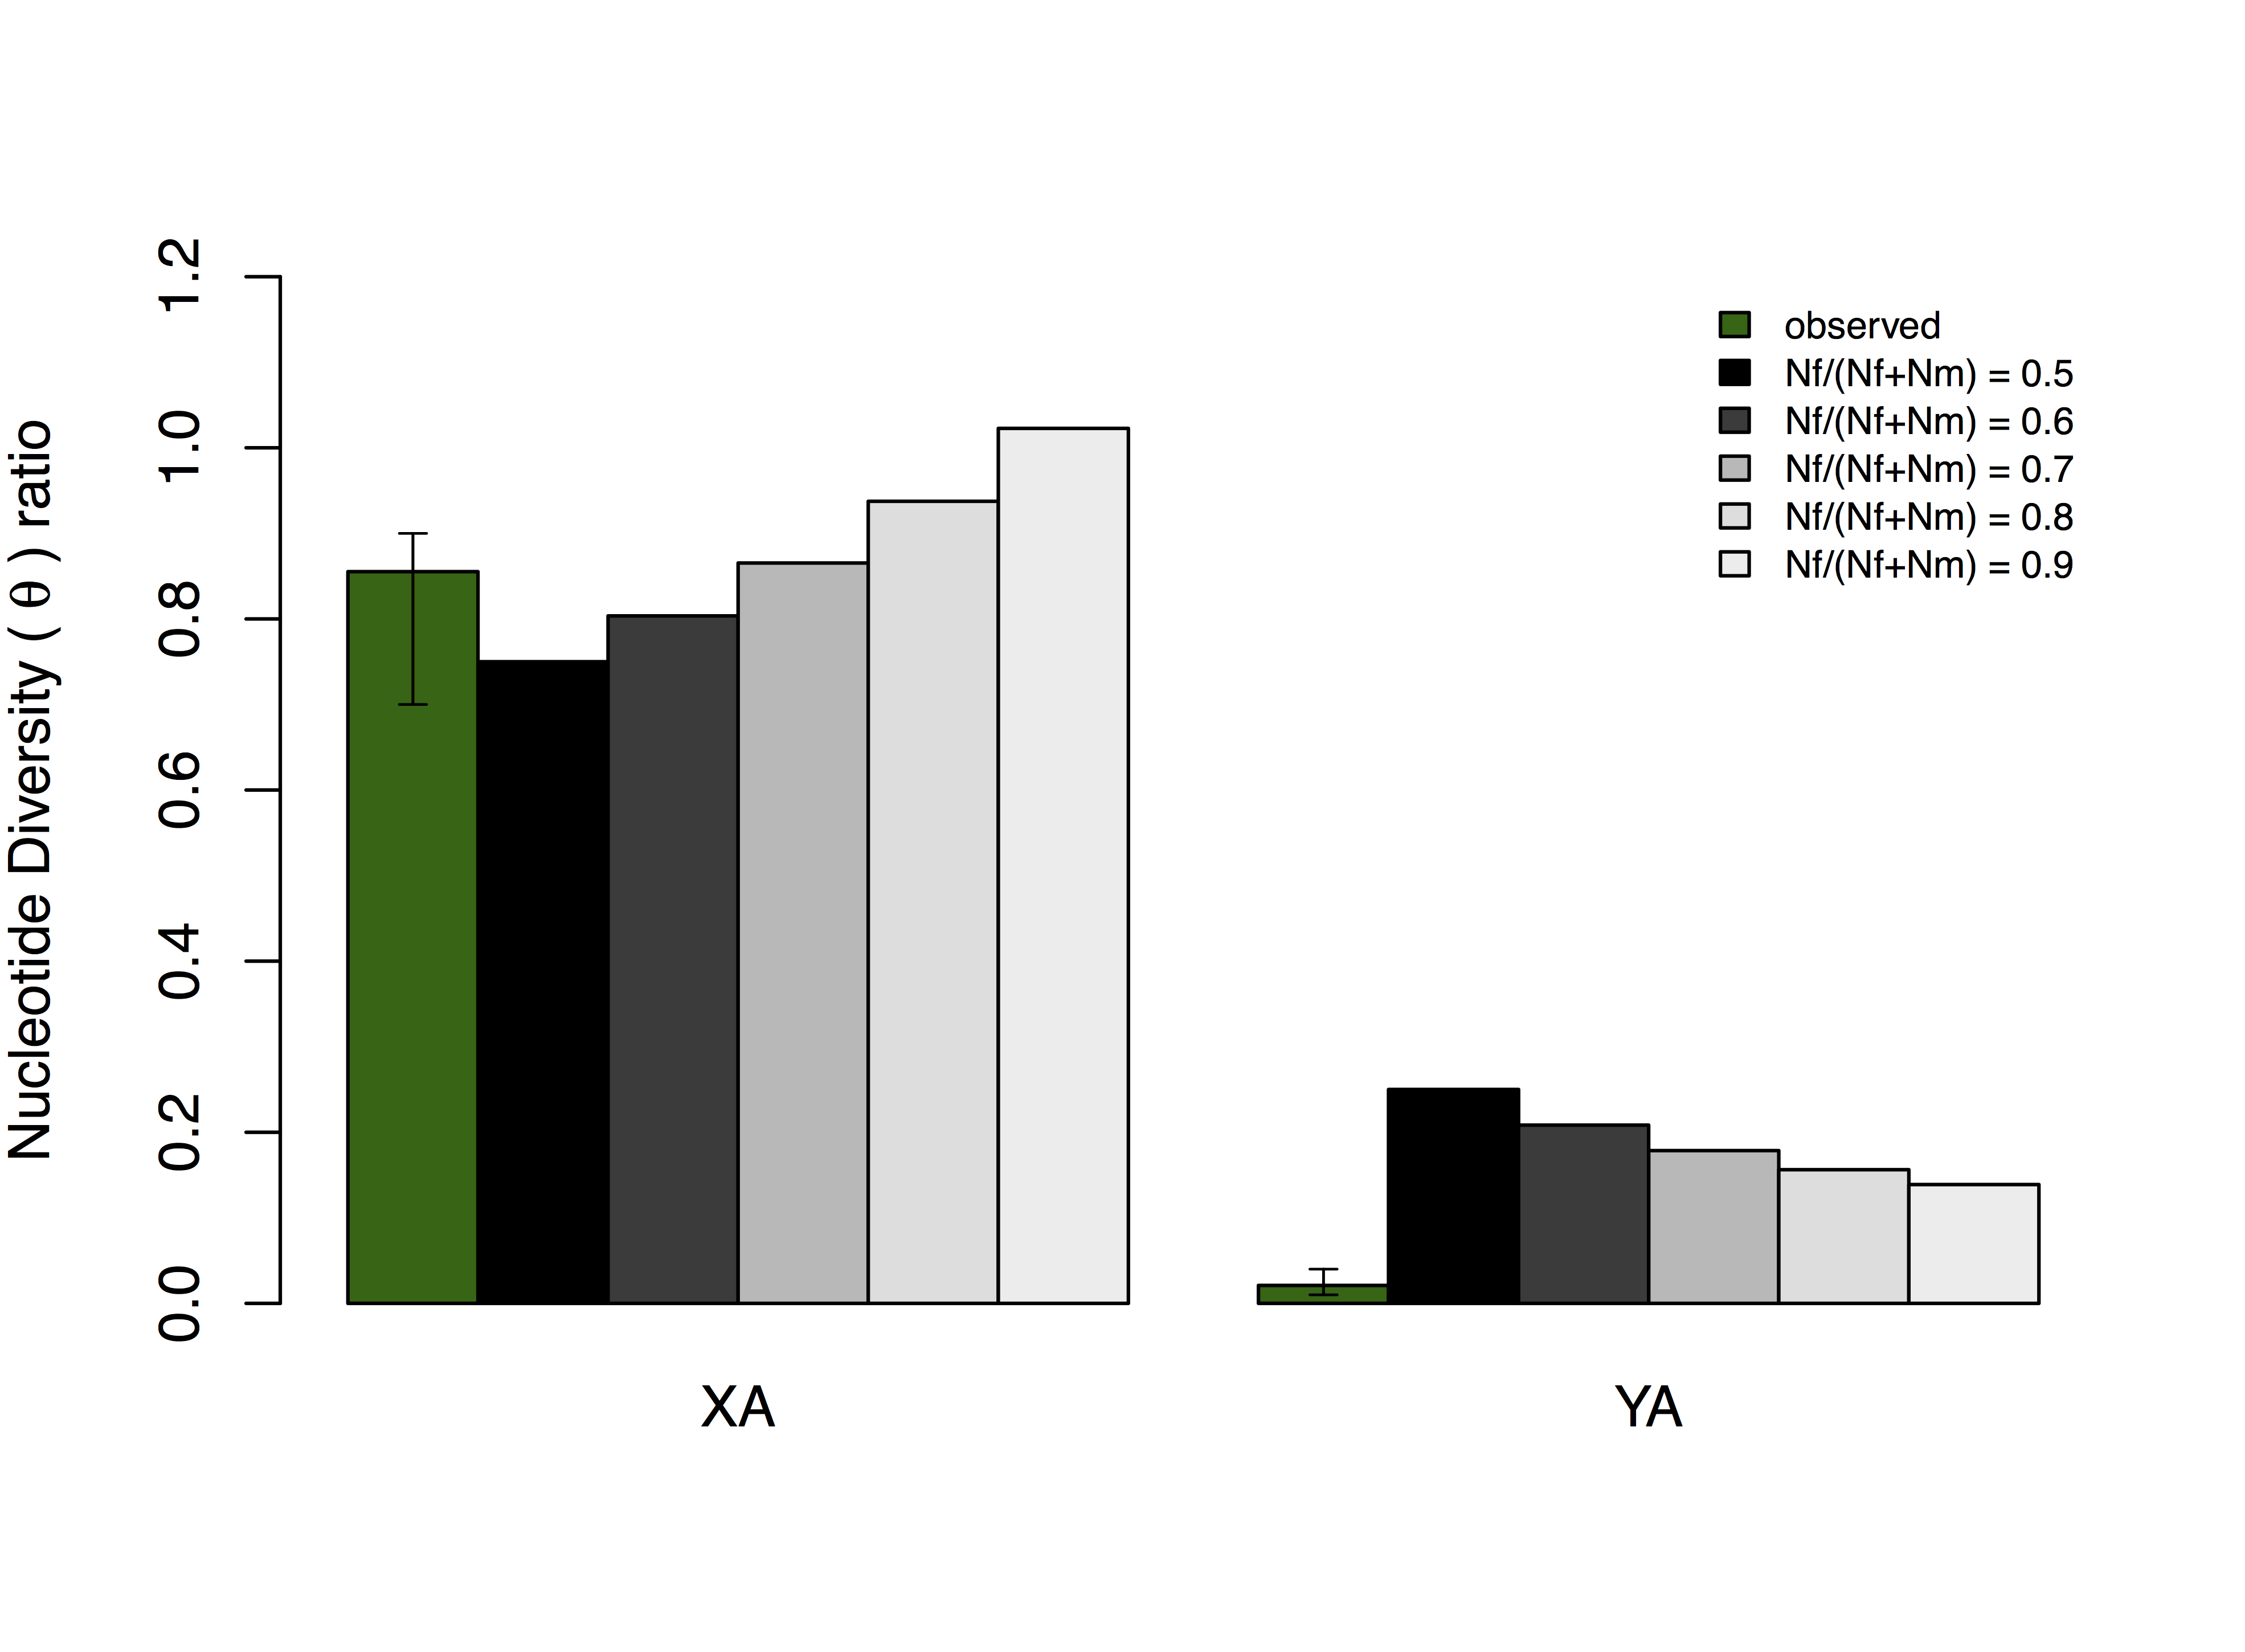
\includegraphics[width=\linewidth]{figure2.jpg}
\caption{new figure coming soon).
}
\label{fig:spectrum}
\end{figure}

In common with most flowering plants we do not have marker-based estimates of the variance in male reproductive success in \textit{R. hastatulus}. However, by comparing our empirical estimates of diversity to predictions from models that jointly predict the effects on diversity of sex ratio bias and male reproductive variance, we evaluated whether these effects could jointly explain the level of Y/A diversity that we observed (see Methods). Conditioning on estimates of sex ratio bias in \textit{R. hastatulus}, ranging from $N_{m}/(N_{m}+N_{f})=0.4$ to $N_{m}/(N_{m}+N_{f})=0.35$ \citep{pickup2013influence}, the predicted Y/A diversity ratio  is approximately 0.2 (Table1, Figure 3). This is significantly lower than our estimated mean Y/A ratio of 0.02 ($\textit{P}<0.0001$), and remains significant even if we consider an upper bound estimate obtained from our likelihood based estimated of the confidence interval. This suggests that the sex ratio effect alone is insufficient to explain our data under the standard sex ratio model.

Assuming that there is extensive variance in male reproductive success (\X), the predicted ratios of Y/A diversity (\X supp) were also significantly higher than our estimates for the empirically estimated sex ratio (\X table) . We also find, however, that purely neutral models in which the sex ratio was highly female-biased (\X), with level of variance in male reproductive success on the order of (\X), predicted a Y/A ratio that could not be rejected (\X). However, because a highly females biased sex ratio is expected to increase the X/A ratio as well, these models simultaneously predicted a range of X/A ratios that were significantly different from what we observed (\X Figure). Thus, our results indicate that the combined effects of sex ratio bias and variance in reproductive success cannot jointly explain our observed levels of X, Y, and autosomal diversity.

\subsection*{Background Selection and Selective Sweeps}


This approach was implemented rather than using analytical predictions of background selection for a few reasons. First,... because the equilibrium background selection model over-predicts the reduction in diversity when there are many linked sites under selection \citep{KaiserCharlesworth}, as is expected to be the case for large Y chromosomes that lack crossing over.


discussion points to make:
- Although we do not exclude the possibility that positive selection has also reduced Y chromosome variability, our simulations suggest that the reduction in diversity arising from purifying selection is sufficient to explain our observed patters of neutral variation.

BGS predictions:
-"Traditionally, the term ‘‘background selection’’ is used to refer both to the general effects of purifying selection on linked neutral diversity as well as to the limiting behavior that emerges when Ns-->inf. "
- "existing theory struggles to predict genetic diversity when many sites experience selection at the same time, which limits our ability to interpret variation in DNA sequence data.". In particular,

- "For non-crossover regions, both with and without gene conversion, there is a rapid initial decline of B with L, but B levels off at a value of  0.015 for > 640 000 sites. B values predicted by the BGS model decrease log-linearly with L"

Very relevant remarks From Good et al.:

- "Here, we have shown that simple behavior emerges in the limit of widespread interference. When fitness variation is composed of many individual mutations, the magnitudes and signs of their fitness effects are relatively unimportant. Instead, molecular evolution is controlled by the variance in fitness within the population over some effectively asexual segment of the genome" " In other words, we cannot conclude that interference is negligible just because ‘‘Nes’’, as inferred from data, is larger than one."

- estimates of "Nes" ignore linkage by fiat under the assumption that sites evolve independently. But these estimates become unreliable precisely when small- and intermediate-effect mutations are most common

- "Individual fitness effects may play a central role in single-site models, but we have shown that global properties like the variance in fitness and the corresponding linkage scale are more relevant for predicting evolution in interfering populations. "

- "We have provided further evidence that even weak purifying selection, when aggregated over a sufficiently large number of sites, can generate strong deviations from neutrality. ""

- "Apart from an overall reduction in polymorphism, the most prominent features of this frequency spectrum include an excess of rare alleles "

- "silent site diversity decays as p=p0*1=Ns, while the shape of the site-frequency spectrum, Qn(i), becomes independent of all underlying parameters."

- " we showed that the reduction in silent site diversity on this chromosome (p=p0*7) is consistent with the parameters Ns<30, NU<300, and NR<0, which fall in the middle of the interference selection regime"

- Indeed, simulations suggest that the effects of HRI on 100,000 linked sites can reduce polymorphism levels by \textasciitilde 30 \% compared to neutral expectations \citep{mcvean2000}, suggesting that HRI is likely important for the evolution of Y chromosomes.

- iven that a large number of sites in the genome likely experience weak purifying selection (\X refs), the "interference" effect on Y chromosomes with suppressed recombination might alone cause a substantial diversity loss.



Classical population genetics fails to account for int
erference between linked mutations, which grows increasingly severe as the density of selected polymorphisms increases.


...there is no general analytical treatment describing the dynamics of interference among many alleles under selection and drift, with variable degrees of selection and linkage. Thus, forward computer simulations are still fundamental to the study of realistic situations.
- dfe for the y is probably still fairly similar to that for the x -- shared genes

- human Y: genes on y are not on X

- 45331 = synsites in observed data after filtering
  - summary stats phased texas autospy

- doesnt matter about coding/non-coding in non-recombining regions? all of those neutral sites are linked


%This reduces their Ne, so that they behave as if they were subject to weaker selection than with free recombination, thereby reducing their effects on linked neutral or nearly neutral variants [9].

%hat genetic variability in these regions can be explained by interference among strongly deleterious mutations

%less effective in influencing the behaviour of neighbouring sites as the number of closely linked sites on a chromosome increases.

%For this chromosome, BGS predicts values of the ratio of neutral diversity to the rest of the genome of  0.1% [9], whereas the observed mean value is  6.5%

%The agreement is reasonably good given the uncertainties involved.

%silent site diversity for 22 genes on the D. miranda neo-Y is
%is  1.2% of the value for their homologues on the recombin- ing neo-X chromosome

% Our observed levels of diversity are essentially at that saturation point, highlighting that we are indeed in a realm where there are a large number of sites subject to purifying selection. So I think we can safely say that, with the caveat about parameter uncertainty, the number of sites under selection is likely to be 800kb or more, consistent with ongoing purifying selection driving down diversity on this chromosome
%This reduces their Ne, so that they behave as if they were subject to weaker selection than with free recombination, thereby reducing their effects on linked neutral or nearly neutral variants [9].

%hat genetic variability in these regions can be explained by interference among strongly deleterious mutations

%less effective in influencing the behaviour of neighbouring sites as the number of closely linked sites on a chromosome increases.

%For this chromosome, BGS predicts values of the ratio of neutral diversity to the rest of the genome of  0.1% [9], whereas the observed mean value is  6.5%

%The agreement is reasonably good given the uncertainties involved.

%silent site diversity for 22 genes on the D. miranda neo-Y is
%is  1.2% of the value for their homologues on the recombin- ing neo-X chromosome

% Our observed levels of diversity are essentially at that saturation point, highlighting that we are indeed in a realm where there are a large number of sites subject to purifying selection. So I think we can safely say that, with the caveat about parameter uncertainty, the number of sites under selection is likely to be 800kb or more, consistent with ongoing purifying selection driving down diversity on this chromosome

%-Although we do not exclude the possibility that positive selection has also reduced Y chromosome variability, our simulations suggest that the reduction in diversity arising from purifying selection is sufficient to explain our observed patters of neutral variation. Given the recent origin of \textit{R. hastatulus} sex chromosomes, our results suggest that the low level of sequence diversity commonly observed on ancient Y chromosomes might evolve relatively quickly after sex chromosomes originate, with selection against deleterious mutations playing an important role during the earliest stages of their evolution.\end{abstract}

%A predicted consequence of a reduction in Ne is an accelerated rate of ¢xation of slightly deleterious substitu- tions, and a reduction in the rate of ¢xation of slightly advantageous mutations (Kimura 1983). Thus we might expect an increased rate of amino-acid replacement rela- tive to silent substitutions on evolving Y chromosomes (provided that su¤cient time has elapsed since the origin of the sex-chromosome system), and more ¢xations of non-preferred versus preferred synonymous substitutions at silent sites in exons (Charlesworth 1996a).

%It is worth noting that our results only apply to the $Y_{1}$ chromosome, as estimates of diversity were calculated for sex-linked genes that were shared between the $XX/XY$ and the $XX/XY_{1}Y_{2}$ sex chromosome systems. Previous work found that both the $Y_{1}$ and the more recently evolved "neo" $Y_{2}$ chromosomes exhibited signs of genetic degeneration, including gene loss, loss of expression, and an accumulation of amino acid-changing mutations \citep{hough2014}, but we cannot say from the present study whether the neo-Y chromosome has also undergone a reduction in diversity. However, the extensive reduction in diversity estimated on the $Y_{1}$ chromosome occurs in each of the three \textit{R. hastatulus} sub-clades (\X Figure 2; Table 1; Figure S2), suggesting that this effect is not population-specific.

% A further interesting aspect of the results from the S. latifolia Y chromosome is that they do not readily ¢t a recent selective sweep. Such an event would eliminate all diversity, so that existing SLY1 polymorphisms must have accumulated since the selective sweep and should thus mostly be at low frequencies (see table 1). However, all six SLY1 polymorphic sites found are non-singletons, and no signi¢cant deviations from neutrality are detectable by standard test statistics (Fu & Li 1993). However, this does not take into account the probable population subdivision in this species. Although a selective sweep eliminating variability throughout the worldwide population of this species seems unlikely, e¡ects of selective sweeps within local populations cannot be excluded.

%because the lack of recombination means that all genes on the Yof any given species share a common genealogy, which limits the amount of information that can be obtained from data on within-species variability.

%This raises the further issue of whether Y-chromosome degeneration is driven mainly by the accumulation of deleterious mutations on the Y or is due to processes turning down the expression of genes on an evolving Y.

%We have focused on the ¢rst of these possibilities, but it might well not completely explain Y degeneration. If mutations of relatively minor ¢tness e¡ects, with Nes not much bigger than 1, become ¢xed more rapidly on a degenerating Ychromosome than on the X, selection pres- sure would develop to reduce the transcription of Y genes, provided that this was compensated for in the hetero- gametic sex by an increased activity of their counterparts on the X.

\section*{Conclusions}


%Our results indicate that highly reduced levels of variability in regions of the Drosophila genome that lack crossing over can largely be explained by the effects of selection on nonsynonymous sites subject to purifying selection of the magnitude indicated by recent work. It seems likely that similar effects will occur in other genomes or genomic regions with low rates of genetic recombination, such as many bacterial genomes, mitochondrial genomes and true Y or W chromosomes that are not completely degenerate, as well as asexual or highly self-fertilizing species.

The observation of widespread degeneration and diversity loss on Y chromosomes illustrates the importance of recombination for maintaining fitness and the genetic variability needed for adaptation (Maynard Smith 1978; Kondrashov 19 93; Barton & Charlesworth 19 9 8). The extensive loss of diversity on a young plant Y chromosome revealed by our study provides a clear example of the .... a large genomic regions that lack recombination.

\section*{Acknowledgments}


\bibliography{bibliography}
\end{document}
